\documentclass[compress,red]{beamer}
\usepackage[utf8]{inputenc}
\usepackage{ucs}
\usepackage{amsmath}
\usepackage{amsfonts}
\usepackage{amssymb}
\usepackage[russian]{babel}
\usepackage{graphicx}
\usepackage{wrapfig}

\usepackage{tikz}
\usepackage{verbatim}

\usepackage{color}
\usepackage{xcolor}
\usepackage{listings}

\usepackage{caption}

\lstset{
language=ruby,
extendedchars=\true,
inputencoding=utf8x,
commentstyle=\itshape,
stringstyle=\bf,
belowcaptionskip=5pt }


\DeclareCaptionFont{white}{\color{white}}
\DeclareCaptionFormat{listing}{\colorbox{gray}{\parbox{\textwidth}{#1#2#3}}}
\captionsetup[lstlisting]{format=listing,labelfont=white,textfont=white}

\usetikzlibrary{calc,trees,positioning,arrows,chains,shapes.geometric,%
    decorations.pathreplacing,decorations.pathmorphing,shapes,%
    matrix,shapes.symbols}

\tikzset{
>=stealth',
  punktchain/.style={
    rectangle, 
    rounded corners, 
    % fill=black!10,
    draw=black, very thick,
    text width=10em, 
    minimum height=3em, 
    text centered, 
    on chain},
  line/.style={draw, thick, <-},
  element/.style={
    tape,
    top color=white,
    bottom color=blue!50!black!60!,
    minimum width=8em,
    draw=blue!40!black!90, very thick,
    text width=10em, 
    minimum height=1.5em, 
    text centered, 
    on chain},
  every join/.style={->, thick,shorten <=1pt},
  decoration={brace},
  tuborg/.style={decorate},
  tubnode/.style={midway, right=2pt},
}

\mode<presentation>

\usetheme{Warsaw}

\definecolor{Red}{rgb}{1,0,0}
\definecolor{Blue}{rgb}{0,0,1}
\definecolor{Green}{rgb}{0,1,0}
\definecolor{magenta}{rgb}{1,0,.6}
\definecolor{lightblue}{rgb}{0,.5,1}
\definecolor{lightpurple}{rgb}{.6,.4,1}
\definecolor{gold}{rgb}{.6,.5,0}
\definecolor{orange}{rgb}{1,0.4,0}
\definecolor{hotpink}{rgb}{1,0,0.5}
\definecolor{newcolor2}{rgb}{.5,.3,.5}
\definecolor{newcolor}{rgb}{0,.3,1}
\definecolor{newcolor3}{rgb}{1,0,.35}
\definecolor{darkgreen1}{rgb}{0, .35, 0}
\definecolor{darkgreen}{rgb}{0, .6, 0}
\definecolor{darkred}{rgb}{.75,0,0}

\xdefinecolor{olive}{cmyk}{0.64,0,0.95,0.4}
\xdefinecolor{purpleish}{cmyk}{0.75,0.75,0,0}

\useoutertheme[subsection=false]{smoothbars}

\title{Информационное общество}
\author{Информатика \\ 8 класс}

%\usecolortheme{dolphin}


\begin{document}
%%титульная страница
\maketitle
%% основные моменты

\section{Мир}
\subsection{Раз}
\begin{frame}
  \begin{center}
    \Huge{Мир меняется...}
  \end{center}
\end{frame}


\subsection{Котэпад}
\begin{frame}[fragile]
\frametitle{Подставка под iPad}
\centerline{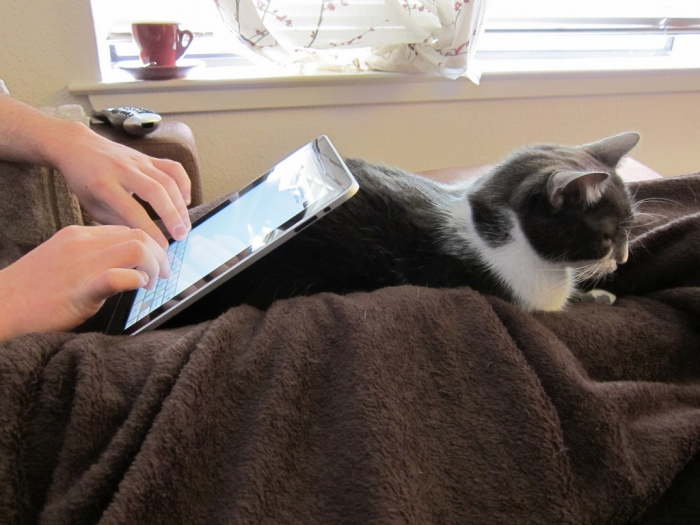
\includegraphics[width=0.8\textwidth]{images/cate.jpg}}
\end{frame}

\subsection{Изменения}
\begin{frame}
  \begin{center}
    \Huge{Изменения происходят}
    
    \Large{во всех сферах жизни}
  \end{center}
\end{frame}

\subsection{Котэпад}
\begin{frame}[fragile]
\frametitle{Подставка под iPad}
\centerline{Ещё 5 лет назад эта картинка вызвала бы недоумение.}
\vspace{0.5cm}
\centerline{
\includegraphics[width=0.7\textwidth]{images/angry_photo.jpg}}
\end{frame}

\section{Информационные революции}
\subsection{Информационные революции}
\begin{frame}[fragile]
  \frametitle{Информационные революции}
  \begin{itemize}
    \item На протяжении всей истории цивилизации произошло несколько \emph{информационных революций} --- скачков в развитии общества, возникших из-за изменений в сфере работы с информацией.
  \end{itemize}
  \begin{enumerate}
    \item Изобретение письменности в Древнем Египте 4000-3000 лет д.н.э.
    \item Изобретение книгопечатания, cередина XVI в.
    \item Изобретение электричества (телеграф, телефон, радио), конец XIX в.
    \item Изобретение компьютера (вторая половина XX в.)
  \end{enumerate}
  
\end{frame}

\subsection{Компьютер}
\begin{frame}
  \begin{center}
    \Huge{Огромный скачок в развитии}
    
    \Large{связан с развитием компьютеров.}
  \end{center}
\end{frame}

\subsection{Святая троица}
\begin{frame}[fragile]
  \frametitle{``Святая троица''}
  \centerline{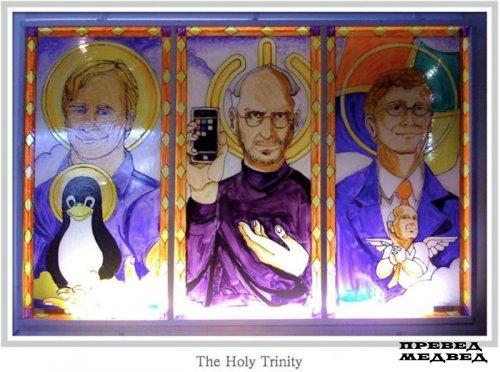
\includegraphics[width=0.8\textwidth]{images/holy_trinity.jpg}}
\end{frame}

\section{Информационное общество}
\subsection{Информационное общество}
\begin{frame}[fragile]
  \frametitle{}
  \begin{itemize}
    \item Четыре информационные революции способствовали появлению \emph{информационного общества}.
    \item Ещё с начала XX века в большинстве развитых стран начал наблюдаться переход от аграрной составляющей (деревня) к производственной и информационной (город).
    \item \emph{Информационное общество} --- это общество, в котором большинство людей занято работой, связанной с созданием, обработкой, хранение и использованием информации.
    \item Большинство современных высококвалифицированных специалистов (юрист, программист, управленец) занимаются интеллектуальным, а не физическим трудом.
  \end{itemize}
\end{frame}

\subsection{Ценности ИО}
\begin{frame}
  \begin{center}
    \Large{Главная ценность ныне --- }
    
    \Huge{информация}
  \end{center}
\end{frame}

\subsection{Плюсы}
\begin{frame}
  \begin{center}
    \Huge{Плюсы и минусы информационного общества}
  \end{center}
\end{frame}

\subsection{Плюсы ИО}
\begin{frame}[fragile]
  \frametitle{Плюсы информационного общества}
  \begin{itemize}
    \item Доступность информации широким слоям населения.
    \item Быстрый и дешёвый способ передачи информации.
    \item Электронные библиотеки и каталоги.
    \item Машинный труд вместо человеческого.
    \item Лёгкость копирования информации.
    \item Отсутствие границ в работе.
  \end{itemize}
\end{frame}

\subsection{Минусы ИО}
\begin{frame}[fragile]
  \frametitle{Минусы информационного общества}
  \begin{itemize}
    \item Информационное изобилие (``О дивный новый мир'', О. Хаксли).
    \item Контроль за людьми.
    \item Нарушение частной жизни и приватности.
    \item Компьютерные вирусы и вредоносное ПО.
    \item Жёлтая пресса.
  \end{itemize}
\end{frame}

\subsection{Жёлтая пресса}
\begin{frame}[fragile]
  \frametitle{Жёлтая пресса}
  \centerline{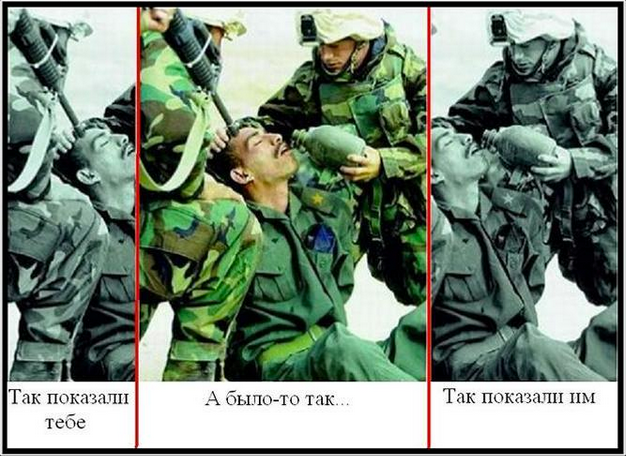
\includegraphics[width=0.8\textwidth]{images/news.png}}
\end{frame}

\subsection{Адекватность восприятия}
\begin{frame}[fragile]
  \frametitle{Адекватность восприятия информации}
  \centerline{
\includegraphics[width=0.8\textwidth]{images/contest.png}}
\end{frame}

\section{Задания}
\subsection{Задания}
\begin{frame}[fragile]
  \frametitle{Задания}
  \begin{enumerate}
    \item Дополните список плюсов и минусов информационного общества своими примерами, три (или больше) плюса и три (или больше) минуса.
    \item Расставьте минусы информационного общества в порядке их важности (согласно вашим представлениям) и объясните, почему вы расставили именно так.
  \end{enumerate}
\end{frame}

\end{document}